\scanpage{29}

$\Gamma=\mathbb G$

\margin{$M\times B'\qquad\operatorname{Ext}(B',DM)$

$\deleted{\operatorname{Hom}(B',\operatorname{Ext}(\unsure{M},\unsure{\mathbb G_m}))}=0$}

\diagram{\begin{tikzcd}[ampersand replacement=\&, row sep=small,column sep=small]
B \& B'\\
M \arrow[u,"i"] \& M' \arrow[u,"i'"']
\end{tikzcd}}
\quad une biext.\inserted{$\mathcal E$} sous $\mathbb G_m$

\diagram{\begin{tikzcd}[ampersand replacement=\&, column sep=small]
B' \arrow[r,"\alpha'"] \& \underline{\operatorname{Ext}}(B,G_m) \arrow[r,no head] \& \underline{\operatorname{Ext}}(M,G_m)
\end{tikzcd}}
nul\quad p.c. $\operatorname{Hom}(B',\overset{\substack{0\\\Vert}}{\underline{\operatorname{Ext}}(M,G_m)}\unsure{)}$

\diagram{\begin{tikzcd}[ampersand replacement=\&, column sep=small]
B \arrow[r,no head,"\alpha"] \& \underline{\operatorname{Ext}}(B',G_m) \arrow[r,no head] \& \underline{\operatorname{Ext}}(M',G_m)
\end{tikzcd}}
nul\quad p.c. $\operatorname{Hom}(B,\underset{\substack{\Vert\\0}}{\underline{\operatorname{Ext}}(M',G_m)}\unsure{)}$

d'où extensions,

\diagram{\begin{tikzcd}[ampersand replacement=\&, column sep=small,row sep=tiny]
\unsure{\bullet|0} \arrow[r,no head] \& DM \arrow[r,"{\unsure{j'}}"] \arrow[d,equal] \& \unsure{G'|C'} \arrow[r,no head,"p'"] \& B' \arrow[r] \& 0\\
 \& T' \& \& \&
\end{tikzcd}}

\margin{\par\noindent\rule{0.8\linewidth}{0.3pt}\par
$\mathcal E_{M,G'}$ est \unsure{canoniqt} splitté par $\rho$
\par\noindent\rule{0.8\linewidth}{0.3pt}\par}

\diagram{\begin{tikzcd}[ampersand replacement=\&, column sep=small,row sep=tiny]
\unsure{\bullet|0} \arrow[r] \& DM' \arrow[r,no head,"{\unsure{j}}"] \arrow[d,equal] \& \unsure{G|C} \arrow[r,no head,"p"] \& B \arrow[r] \& 0\\
 \& T \& \& \&
\end{tikzcd}}

\margin{$\mathcal E_{G,M'}$ est can. splitté $\rho'$
\par\noindent\rule{0.8\linewidth}{0.3pt}\par}

\uline{\unsure{Exemple}} si \deleted{\unsure{par}} $\uline{\alpha'}$ \deleted{\unsure{était}} \inserted{\unsure{est}} un isom, alors $i'$ \unsure{revient à se donner}

un
\diagram{\begin{tikzcd}[ampersand replacement=\&, column sep=small]
i'\in\unsure{\operatorname{Hom}}(M',\underline{\operatorname{Ext}}(B,G_m)) \& \operatorname{Biext}(B,M';G_m) \arrow[l,"\sim"'] \& \deleted{\unsure{\operatorname{Hom}}}\inserted{\operatorname{Ext}(B,D(M'))} \arrow[l,"\sim"']
\end{tikzcd}}

\margin{si $\unsure{\operatorname{Ext}}(M',\underline{\operatorname{Hom}}(B,G_m))=0$

p.ex.
\figure{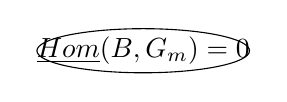
\begin{tikzpicture}[baseline=(t.base)]\node (t) {$\underline{\operatorname{Hom}}(B,G_m)=0$};\draw (0,0) ellipse (1.35 and 0.28);\end{tikzpicture}}}

\margin{si $\operatorname{Hom}(B,\underset{\substack{\Vert\\0}}{\underline{\operatorname{Ext}}(M',G_m)}\unsure{)}$ p.ex.
\figure{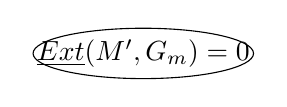
\begin{tikzpicture}[baseline=(t.base)]\node (t) {$\underline{\operatorname{Ext}}(M',G_m)=0$};\draw (0,0) ellipse (1.40 and 0.32);\end{tikzpicture}}}

\unsure{aussi} \unsure{pour}. Donc la donnée de $i'$ \unsure{équivaut à} celle de l'ext. $G$. Et réciproquement.

Considérons l'image inverse\inserted{\figure{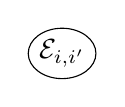
\begin{tikzpicture}[baseline=(t.base)]\node (t) {$\mathcal E_{i,i'}$};\draw (0,0) ellipse (0.43 and 0.32);\end{tikzpicture}}}
de $\mathcal E$ sur $(M,M')$. Alors des \unsure{splittages}\inserted{$\unsure{\rho_i}$} de cette biextension correspondent aux hom $j$ de $M$ dans $G$ relevant $i$, \unsure{aux hom}\,$j'$ de $M'$ dans $G'$ relev. de $i'$.

\diagram{\begin{tikzcd}[ampersand replacement=\&, row sep=tiny,column sep=small]
M \arrow[r,no head] \& G \arrow[r,no head] \& B\\
M' \arrow[r,no head] \& G' \arrow[r,no head] \& B'
\end{tikzcd}}

\figure{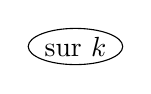
\begin{tikzpicture}[baseline=(t.base)]\node (t) {\deleted{\unsure{sur $k$}}};\draw (0,0) ellipse (0.60 and 0.23);\end{tikzpicture}}

\inserted{Deux relèvements} \deleted{\unsure{si}} $j$ et $j'$ \deleted{\unsure{se}} \unsure{se correspondent ainsi},

\deleted{\unsure{Alors on trouve un} splitt. $\sigma$ canonique \deleted{$\unsure{\sigma'}$} de $\mathcal E_{G,M'}$ et un splitt. $\sigma'$ canonique de $\mathcal E_{M,G'}$, ces deux splittages coïncident sur $M,M'$ avec le splittage \unsure{donné} $h$ de $\mathcal E_{M,M'}$.}

ssi les deux splittages de $\mathcal E_{M,M'}$, déduits d'une part du splittage $\rho$ de $\mathcal E_{M,G'}$ \unsure{et de} $j':M'\longrightarrow G'$, d'autre part du splittage $\rho'$ de $\mathcal E_{G,M'}$ et de $j:M\mathbin{-}G$, coïncident.

\margin{28}
